\documentclass[a4paper,UTF8]{article}
\usepackage{amsmath}
\usepackage{amssymb}
\usepackage{amsthm}
\usepackage{bm}
\usepackage{color}
\usepackage{ctex}
\usepackage{enumerate}
\usepackage[margin=1.25in]{geometry}
\usepackage{graphicx}
\usepackage{hyperref}
\usepackage{tcolorbox}
\usepackage{algorithm}
\usepackage{algorithmic}
\usepackage{pythonhighlight}
\theoremstyle{definition}
\newtheorem*{solution}{Solution}
\newtheorem*{prove}{Proof}
\newcommand{\indep}{\rotatebox[origin=c]{90}{$\models$}}
\usepackage{multirow}              

\setlength{\evensidemargin}{.25in}
\setlength{\textwidth}{6in}
\setlength{\topmargin}{-0.5in}
\setlength{\topmargin}{-0.5in}
% \setlength{\textheight}{9.5in}
%%%%%%%%%%%%%%%%%%此处用于设置页眉页脚%%%%%%%%%%%%%%%%%%
\usepackage{fancyhdr}                                
\usepackage{lastpage}                                           
\usepackage{layout}                                             
\footskip = 12pt 
\pagestyle{fancy}                    % 设置页眉                 
\lhead{2020年春季}                    
\chead{机器学习导论}                                                
% \rhead{第\thepage/\pageref{LastPage}页} 
\rhead{作业一}                                                                                               
\cfoot{\thepage}                                                
\renewcommand{\headrulewidth}{1pt}  			%页眉线宽,设为0可以去页眉线
\setlength{\skip\footins}{0.5cm}    			%脚注与正文的距离           
\renewcommand{\footrulewidth}{0pt}  			%页脚线宽,设为0可以去页脚线

\makeatletter 									%设置双线页眉                                        
\def\headrule{{\if@fancyplain\let\headrulewidth\plainheadrulewidth\fi%
		\hrule\@height 1.0pt \@width\headwidth\vskip1pt	%上面线为1pt粗  
		\hrule\@height 0.5pt\@width\headwidth  			%下面0.5pt粗            
		\vskip-2\headrulewidth\vskip-1pt}      			%两条线的距离1pt        
	\vspace{6mm}}     								%双线与下面正文之间的垂直间距              
\makeatother  


\begin{document}
	\title{机器学习导论\\
		习题六}
	\author{171830635, 俞星凯, yuxk@smail.nju.edu.cn}
	\maketitle
	
	
	\section*{学术诚信}
	
	本课程非常重视学术诚信规范,助教老师和助教同学将不遗余力地维护作业中的学术诚信规范的建立。希望所有选课学生能够对此予以重视。\footnote{参考尹一通老师\href{http://tcs.nju.edu.cn/wiki/}{高级算法课程}中对学术诚信的说明。}
	
	\begin{tcolorbox}
		\begin{enumerate}
			\item[(1)] 允许同学之间的相互讨论,但是{\color{red}\textbf{署你名字的工作必须由你完成}},不允许直接照搬任何已有的材料,必须独立完成作业的书写过程;
			\item[(2)] 在完成作业过程中,对他人工作(出版物、互联网资料)中文本的直接照搬(包括原文的直接复制粘贴及语句的简单修改等)都将视为剽窃,剽窃者成绩将被取消。{\color{red}\textbf{对于完成作业中有关键作用的公开资料,应予以明显引用}};
			\item[(3)] 如果发现作业之间高度相似将被判定为互相抄袭行为,{\color{red}\textbf{抄袭和被抄袭双方的成绩都将被取消}}。因此请主动防止自己的作业被他人抄袭。
		\end{enumerate}
	\end{tcolorbox}
	
	\section*{作业提交注意事项}
	\begin{tcolorbox}
		\begin{enumerate}
			\item[(1)] 请在\LaTeX 模板中{\color{red}\textbf{第一页填写个人的姓名、学号、邮箱信息}};
			\item[(2)] 本次作业需提交该pdf文件、问题3可直接运行的源码(BoostMain.py, RandomForestMain.py,不需要提交数据集),将以上三个文件压缩成zip文件后上传。zip文件格式为{\color{red}\textbf{学号.zip}},例如170000001.zip;pdf文件格式为{\color{red}\textbf{学号\_姓名.pdf}},例如170000001\_张三.pdf。
			\item[(3)] 未按照要求提交作业,或提交作业格式不正确,将会{\color{red}\textbf{被扣除部分作业分数}};
			\item[(4)] 本次作业提交截止时间为{\color{red}\textbf{6月11日23:59:59。本次作业不允许缓交,截止时间后不接收作业,本次作业记零分}}。
		\end{enumerate}
	\end{tcolorbox}
	
	\newpage




\section{\textbf{[25pts]} Bayesian Network}
贝叶斯网(Bayesian Network)是一种经典的概率图模型,请学习书本7.5节内容回答下面的问题:

(1) \textbf{[5pts]} 请画出下面的联合概率分布的分解式对应的贝叶斯网结构:
\begin{equation*}
\Pr(A, B, C, D, E, F, G) = \Pr(A)\Pr(B)\Pr(C)\Pr(D|A)\Pr(E|A)\Pr(F|B, D)\Pr(G|D, E)
\end{equation*}

(2) \textbf{[5pts]} 请写出图\ref{fig-DAG}中贝叶斯网结构的联合概率分布的分解表达式。
\begin{figure}[h]
\centering
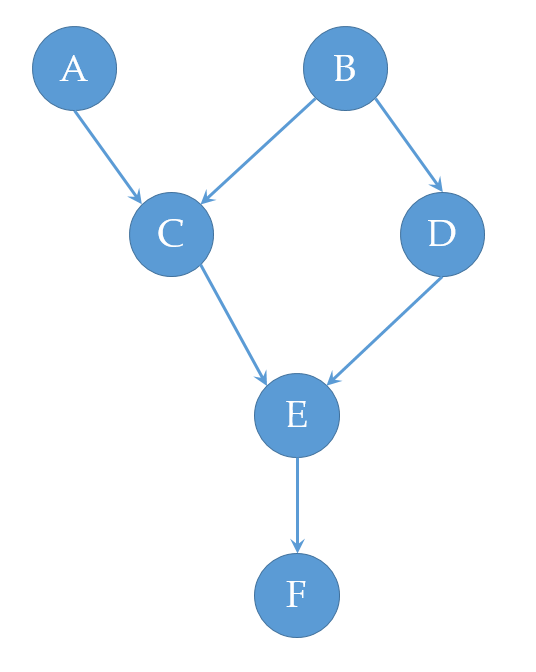
\includegraphics[scale=0.3]{bayes_net.png}
\caption{题目1-(2)有向图}
\label{fig-DAG}
\end{figure}

(3) \textbf{[15pts]} 基于第(2)问中的图\ref{fig-DAG}, 请判断表格\ref{table:DAG}中的论断是否正确。首先需要作出对应的道德图,并将下面的表格填完整。
\begin{table}[h]
\centering
\caption{判断表格中的论断是否正确}
\label{table:DAG}
\begin{tabular}{c|l|c||c|l|c}\hline
序号   		& 		关系  			& True/False 	& 序号   	& 		关系  			& True/False \\ \hline
1			&	$A \indep B$ 		    & 			    & 7  		& 	$F \perp B|C$ 		& 			 \\
2			&	$A \perp B|C$ 	    & 			    & 8  		& 	$F \perp B|C, D$ 	& 			 \\
3			&	$C \indep D $		    & 			    & 9  		& 	$F \perp B|E$ 		& 			 \\
4			&	$C \perp D|E$ 	    & 			    & 10  		& 	$A \indep F $			& 			 \\
5			&	$C \perp D|B, F$     & 			    & 11  		& 	$A \perp F|C$ 		& 			 \\
6			&	$F \indep B $		    & 			    & 12  		& 	$A \perp F|D$ 		& 			 \\ \hline
\end{tabular}
\end{table}

\begin{solution}
	~\\
	\begin{enumerate}[(1)]
		\item 
		根据联合概率表达式可以得到有向边:
		\[
		A \rightarrow D,A \rightarrow E,B \rightarrow F,D \rightarrow F,D \rightarrow G,E \rightarrow G
		\]
		\begin{figure}[h]
			\centering
			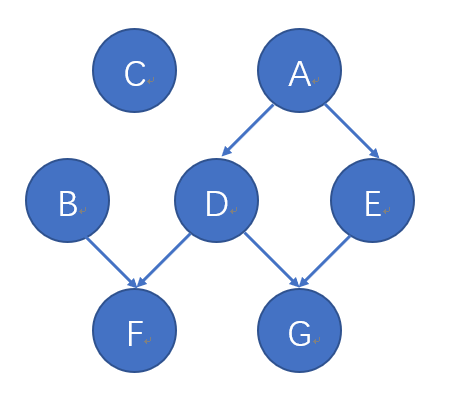
\includegraphics[scale=0.3]{mybayes.png}
		\end{figure}
	
		\item 
		根据有向边可以写出联合概率表达式:
		\[
		Pr(A,B,C,D,E,F)=Pr(A)Pr(B)Pr(C|A,B)Pr(D|B)Pr(E|C,D)Pr(F|E)
		\]
		
		\item 
		贝叶斯网对应道德图:
		\begin{figure}[h]
			\centering
			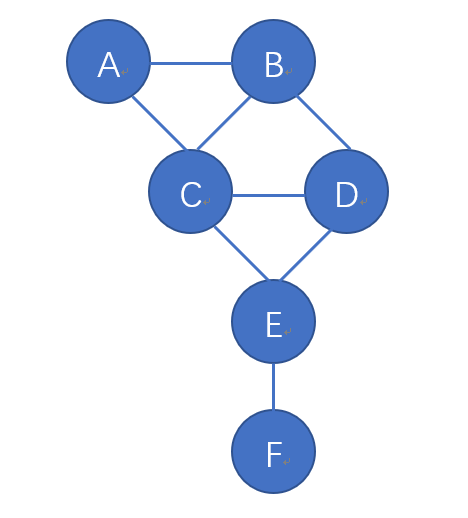
\includegraphics[scale=0.3]{moral.png}
		\end{figure}
		\begin{table}[h]
			\centering
			\begin{tabular}{c|l|c||c|l|c}\hline
				序号   		& 		关系  			& True/False 	& 序号   	& 		关系  			& True/False \\ \hline
				1			&	$A \indep B$ 		    & True			    & 7  		& 	$F \perp B|C$ 		& False			 \\
				2			&	$A \perp B|C$ 	    & False			    & 8  		& 	$F \perp B|C, D$ 	& True			 \\
				3			&	$C \indep D $		    & False			    & 9  		& 	$F \perp B|E$ 		& True			 \\
				4			&	$C \perp D|E$ 	    & False			    & 10  		& 	$A \indep F $			& False			 \\
				5			&	$C \perp D|B, F$     & False			    & 11  		& 	$A \perp F|C$ 		& False			 \\
				6			&	$F \indep B $		    & False			    & 12  		& 	$A \perp F|D$ 		& False			 \\ \hline
			\end{tabular}
		\end{table}
	\end{enumerate}
\end{solution}



\section{\textbf{[35$+$10pts]} Theoretical Analysis of $k$-means Algorithm}
给定样本集$\mathcal{D}=\left\{\mathbf{x}_{1}, \mathbf{x}_{2}, \ldots, \mathbf{x}_{n}\right\}$, $k$-means聚类算法希望获得簇划分$\mathcal{C}=\left\{C_{1}, C_{2}, \cdots, C_{k}\right\}$
使得最小化欧式距离
\begin{align} \label{eq1}
J\left(\gamma, \mu_{1}, \ldots, \mu_{k}\right)=\sum_{i=1}^{n} \sum_{j=1}^{k} \gamma_{i j}\left\|\mathbf{x}_{i}-\mu_{j}\right\|^{2}
\end{align}

其中$\mu_{1}, \ldots, \mu_{k}$为$k$个簇的中心(means), 
 $\gamma \in \mathbb{R}^{n \times k}$为指示矩阵(indicator matrix)定义如
下:若$\mathbf{x}_{i}$属于第j个簇, 则$\gamma_{i j}=1$, 否则为0,则最经典的$k$-means聚类算法流程如算法\ref{alg:alg1}中所示

{\begin{algorithm}[h]
		\caption{ $k-$means Algorithm }
		\label{alg:alg1}
		\begin{algorithmic}[1]{
				\STATE Initialize $\mu_{1}, \ldots, \mu_{k}$;
				\REPEAT
				\STATE {\bf{Step 1:}} Decide the class memberships of $\left\{\mathbf{x}_{i}\right\}_{i=1}^{n}$ by assigning each of them
				to its nearest cluster center.
				
				\begin{align}\gamma_{i j}=\left\{\begin{array}{ll}
				1, & \left\|\mathbf{x}_{i}-\mu_{j}\right\|^{2} \leq\left\|\mathbf{x}_{i}-\mu_{j^{\prime}}\right\|^{2}, \forall j^{\prime} \\
				0, & \text { otherwise }
				\end{array}\right.\end{align}
				\STATE {\bf{Step 2:}} For each $j \in\{1, \cdots, k\}$, recompute $\mu_j$ using the updated 
$\gamma$ to be	the center of mass of all points in $C_j$ :
			\begin{align}\mu_{j}=\frac{\sum_{i=1}^{n} \gamma_{i j} \mathbf{x}_{i}}{\sum_{i=1}^{n} \gamma_{i j}}\end{align}	
		
				\UNTIL the objective function J no longer changes;}
		\end{algorithmic}
		
\end{algorithm}}


(1) \textbf{[5pts]} 试证明, 在算法\ref{alg:alg1}中, Step 1和Step 2都会使目标函数J的值降低.

(2) \textbf{[5pts]} 试证明, 算法\ref{alg:alg1}会在有限步内停止。


(3) \textbf{[10pts]} 试证明, 目标函数J的最小值是关于$k$的非增函数, 其中$k$是聚类簇的数目。

(4) \textbf{[15pts]} 记$\hat{\mathbf{x}}$为$n$个样本的中心点, 定义如下变量,

\begin{table}[h]
	\centering
	\begin{tabular}{l}
		$T(X)=\sum_{i=1}^{n}\left\|\mathbf{x}_{i}-\hat{\mathbf{x}}\right\|^{2} / n$  \\
		$W_{j}(X)=\sum_{i=1}^{n} \gamma_{i j}\left\|\mathbf{x}_{i}-\mu_{j}\right\|^{2} / \sum_{i=1}^{n} \gamma_{i j}$  \\
		$B(X)=\sum_{j=1}^{k} \frac{\sum_{i=1}^{n} \gamma_{i j}}{n}\left\|\mu_{j}-\hat{\mathbf{x}}\right\|^{2}$  \\
	\end{tabular}
\end{table}

试探究以上三个变量之间有什么样的等式关系?基于此请证明, $k$-means聚类算法可以认为是在最小化$W_j(X)$的加权平均, 同时最大化$B(X)$.


(5) \textbf{[Bonus 10pts]}在公式\ref{eq1}中, 我们使用$\ell_{2^{-}}$范数来度量距离(即欧式距离), 下面我们考虑使用$\ell_{1^{-}}$范数来度量距离
\begin{equation}
\label{eq4}
J^{\prime}\left(\gamma, \mu_{1}, \ldots, \mu_{k}\right)=\sum_{i=1}^{n} \sum_{j=1}^{k} \gamma_{i j}\left\|\mathbf{x}_{i}-\mu_{j}\right\|_{1}
\end{equation}
\begin{itemize}
	\item 请仿效算法\ref{alg:alg1},给出新的算法(命名为$k-$means-$\ell_{1}$算法)以优化公式\ref{eq4}中的目标函数$J^{\prime}$. 
	\item 当样本集中存在少量异常点\href{https://en.wikipedia.org/wiki/Outlier}{(outliers)}时, 上述的$k-$means-$\ell_{2}$和$k-$means-$\ell_{1}$算法,	我们应该采用哪种算法?即哪个算法具有更好的鲁棒性?请说明理由。
\end{itemize}


\begin{solution}
	~\\
	\begin{enumerate}[(1)]
		\item 
		在Step 1中,记$x_i(1\leq i\leq n)$与第$g_i$个簇中心距离最近。
		\[
		J(\gamma,\mu_1,\cdots,\mu_k) \geq \sum_{i=1}^{n}\sum_{j=1}^{k}\gamma_{ij}\Vert x_i-\mu_{g_i} \Vert^2=\sum_{i=1}^{n}\sum_{j=1}^{k}\Vert x_i-\mu_{g_i} \Vert^2
		\]
		当$\mu_i(1\leq i\leq k)$给定时,$\gamma_{ij}=\mathbb{I}(j=g_i)$可以最小化$J$。\\
		在Step2中,计算$J$对$\mu_j$偏导
		\begin{align*}
		\frac{\partial J}{\partial \mu_j}
		&=\frac{\sum_{j=1}^{k}\sum_{i=1}^{n}\gamma_{ij}\Vert x_i-\mu_j \Vert^2}{\partial \mu_j}\\
		&=\frac{\sum_{i=1}^{n}\gamma_{ij}\Vert x_i-\mu_j \Vert^2}{\partial \mu_j}\\
		&=2\sum_{i=1}^n\gamma_{ij}(\mu_j-x_i)
		\end{align*}
		令偏导为0,得出
		\[\mu_j=\frac{\sum_{i=1}^n\gamma_{ij}x_i}{\sum_{i=1}^n\gamma_{ij}}\]
		当$\gamma_{ij}(1\leq i\leq n,1\leq j\leq k)$给定时,$\mu_j$按照上式取值可以最小化$J$。\\
		因此,Step1和Step2都会使$J$的值降低。
		
		\item 
		显然$J$存在下界0,并且算法使得$J$单调递减,所以算法一定收敛。
		
		\item 
		已知当簇的数量为$k$时的最优$\gamma$和$\mu$,当簇的数量为$k+1$时,令第$k+1$个簇中心$\mu'_{k+1}=x_n$,并且$x_n$属于第$k+1$个簇中心$\gamma'_{n,k+1}=1$,其余$\gamma'_{ij}(1\leq i\leq n-1,1\leq j\leq k)$和$\mu'_j(1\leq j\leq k)$不变,于是
		\begin{align*}
		J(\gamma',\mu'_1,\cdots,\mu'_{k+1})
		&=\sum_{i=1}^{n}\sum_{j=1}^{k+1}\gamma'_{ij}\Vert x_i-\mu'_j \Vert^2\\
		&=\sum_{i=1}^{n-1}\sum_{j=1}^{k+1}\gamma'_{ij}\Vert x_i-\mu'_j \Vert^2+\sum_{j=1}^{k+1}\gamma'_{ij}\Vert x_n-\mu'_j \Vert^2\\
		&=\sum_{i=1}^{n-1}\sum_{j=1}^{k}\gamma_{ij}\Vert x_i-\mu_j \Vert^2+\Vert x_n-\mu'_{k+1} \Vert^2\\
		&=\sum_{i=1}^{n-1}\sum_{j=1}^{k}\gamma_{ij}\Vert x_i-\mu_j \Vert^2\\
		&\leq J(\gamma,\mu_1,\cdots,\mu_k)
		\end{align*}
		所以$J$的最小值是关于$k$的非增函数。
		
		\item 
		%令$S_j=\{x_i|r_{ij}=1\}(1\leq j\leq k)$
		\begin{align*}
		nT(X)&=\sum_{i=1}^n\Vert x_i-\hat{x} \Vert^2\\
		%&=\sum_{i=1}^n\Vert x_i-\mu_{g_i}+\mu_{g_i}-\hat{x} \Vert^2\\
		&=\sum_{i=1}^n\sum_{j=1}^k\gamma_{ij}\Vert x_i-\hat{x} \Vert^2\\
		&=\sum_{i=1}^n\sum_{j=1}^k\gamma_{ij}\Vert x_i-\mu_j+\mu_j-\hat{x} \Vert^2\\
		%&=\sum_{i=1}^n\Vert x_i-\mu_{g_i} \Vert^2+\sum_{i=1}^n\Vert \mu_{g_i}-\hat{x} \Vert^2+2\sum_{i=1}^n(x_i-\mu_{g_i})(\mu_{g_i}-\hat{x})\\
		&=\sum_{j=1}^k\sum_{i=1}^n\gamma_{ij}\Vert x_i-\mu_j \Vert^2+\sum_{j=1}^k\sum_{i=1}^n\gamma_{ij}\Vert\mu_j-\hat{x} \Vert^2+2\sum_{j=1}^k(\mu_j-\hat{x})\sum_{i=1} ^n\gamma_{ij}(x_i-\mu_j)\\
		&=\sum_{j=1}^k\sum_{i=1}^n\gamma_{ij}W_j(X)+nB(X)+0
		\end{align*}
		因为$J=\sum_{j=1}^k\sum_{i=1}^n\gamma_{ij}W_j(X)$,所以$k$-means算法最小化$J$等价于最小化$W_j(X)$的加权平均。同时$J$与$nB(X)$之和为定值,最小化$J$等价于最大化$B(X)$。
		
		\item 
		令$S_j=\{x_i|\gamma_{ij}=1\}$,即属于第$j$个簇的样本集。
		{\begin{algorithm}[H]
				\caption{ $k-$means Algorithm }
				\label{alg:alg2}
				\begin{algorithmic}[1]{
						\STATE Initialize $\mu_{1}, \ldots, \mu_{k}$;
						\REPEAT
						\STATE {\bf{Step 1:}} Decide the class memberships of $\left\{\mathbf{x}_{i}\right\}_{i=1}^{n}$ by assigning each of them
						to its nearest cluster center.
						
						\begin{align}\gamma_{i j}=\left\{\begin{array}{ll}
						1, & \left\|\mathbf{x}_{i}-\mu_{j}\right\|_1 \leq\left\|\mathbf{x}_{i}-\mu_{j^{\prime}}\right\|_1, \forall j^{\prime} \\
						0, & \text { otherwise }
						\end{array}\right.\end{align}
						\STATE {\bf{Step 2:}} For each $j \in\{1, \cdots, k\}$, recompute $\mu_j$ using the updated 
						$\gamma$ to be	the center of mass of all points in $C_j$ :
						\begin{align}\mu_{j}=median_{\mathbf{x}\in S_j}(\mathbf{x})\end{align}	
						
						\UNTIL the objective function J no longer changes;}
				\end{algorithmic}
		\end{algorithm}}
		k-means-$\ell_{1}$算法具有更好鲁棒性,因为当异常点数量不多时,中值操作可以屏蔽它们的影响,而均值操作则会被极大影响。
	\end{enumerate}
\end{solution}


\section{[40pts] Coding: Ensemble Methods }

本次实验中我们将结合两种经典的集成学习思想:Boosting和Bagging,对集成学习方法进行实践。本次实验选取UCI数据集Adult,此数据集为一个二分类数据集,具体信息可参照\href{http://archive.ics.uci.edu/ml/datasets/Adult}{链接},为了方便大家使用数据集,已经提前对数据集稍作处理,并划分为训练集和测试集,数据集文件夹为adult\_dataset。

由于Adult是一个类别不平衡数据集,本次实验选用AUC作为评价分类器性能的评价指标,可调用\href{http://scikit-learn.org/stable/modules/generated/sklearn.metrics.roc_auc_score.html}{sklearn算法包}对AUC指标进行计算。

\begin{enumerate}[(1)]
	\item 本次实验要求使用Python3编写,要求代码分布于两个文件中,BoostMain.py, RandomForestMain.py ,调用这两个文件就能完成一次所实现分类器的训练和测试;
	
	\item \textbf{[35pts]} 本次实验要求编程实现如下功能:
	
	\begin{itemize}
		\item \textbf{[10pts]} 结合教材8.2节中图8.3所示的算法伪代码实现AdaBoost算法,基分类器选用决策树,基分类器可调用sklearn中\href{http://scikit-learn.org/stable/modules/generated/sklearn.tree.DecisionTreeClassifier.html}{决策树}的实现;
		\item \textbf{[10pts]} 结合教材8.3.2节所述,实现随机森林算法,基分类器仍可调用sklearn中决策树的实现,也可以手动实现,在实验报告中请给出随机森林的算法伪代码;
		\item \textbf{[10pts]} 结合AdaBoost和随机森林的实现,调查基学习器数量对分类器训练效果的影响 ,具体操作如下:分别对AdaBoost和随机森林,给定基分类器数目,在训练数据集上用5折交叉验证得到验证AUC评价。在实验报告中用折线图的形式报告实验结果,折线图横轴为基分类器数目,纵轴为AUC指标,图中有两条线分别对应AdaBoost和随机森林,基分类器数目选取范围请自行决定;
		\item \textbf{[5pts]} 根据参数调查结果,对AdaBoost和随机森林选取最好的基分类器数目,在训练数据集上进行训练,在实验报告中报告在测试集上的AUC指标;
	\end{itemize}
	
	\item \textbf{[5pts]} 在实验报告中,除了报告上述要求报告的内容外还需要展现实验过程,实验报告需要有层次和条理性,能让读者仅通过实验报告便能了解实验的目的,过程和结果。
	
\end{enumerate}

\noindent{\textbf{实验报告.}}
~\\
实现一个类AdaBoost封装算法,基学习器使用sklearn中的决策分类树。\\
首先需要保存基学习器个数$n$和决策树参数$kwargs$。
\begin{python}
def __init__(self, n, **kwargs):
	self.n = n
	self.kwargs = kwargs
\end{python}
然后实现$fit()$方法,重复训练新的决策树,计算对应权重$alpha$,并迭代样本权重$w$。
\begin{python}
def fit(self, X, y):
	self.clfs = []
	self.alphas = []
	w = np.ones_like(y) / y.shape[0]
	for i in range(self.n):
		clf = DecisionTreeClassifier(max_depth=1, **self.kwargs)
		clf.fit(X, y, sample_weight=w)
		z = clf.predict(X)
		err = 1 - accuracy_score(y, z, sample_weight=w)
		if err > 0.5:
			break
		alpha = 0.5 * np.log((1-err) / err)
		w *= np.exp(-alpha * y * z)
		w /= w.sum()
		self.clfs.append(clf)
		self.alphas.append(alpha)
	return self
\end{python}
最后实现$predict()$方法,将各决策树预测结果根据$alpha$线性组合,求出符号即为预测结果。
\begin{python}
def predict(self, X):
	y = np.zeros(X.shape[0])
	for alpha, clf in zip(self.alphas, self.clfs):
		y += alpha * clf.predict(X)
	return np.sign(y)
\end{python}
实现一个类RandomForest封装算法,同样需要保存基学习器个数$n$和决策树参数$kwargs$,不再赘述。直接看$fit()$方法,需要限制每次划分特征是从随机特征子集中选择的,并且训练集基于Bootstrap生成。
\begin{python}
def fit(self, X, y):
	self.clfs = []
	for i in range(self.n):
		clf = DecisionTreeClassifier(max_features='log2', **self.kwargs)
		idx = np.random.choice(np.arange(y.shape[0]), y.shape[0])
		clf.fit(X[idx], y[idx])
		self.clfs.append(clf)
	return self
\end{python}
$predict()$实现类似AdaBoost,区别是不需要加权。
\begin{python}
def predict(self, X):
	y = np.zeros(X.shape[0])
	for clf in self.clfs:
		y += clf.predict(X)
	return np.sign(y)
\end{python}
在训练集上的5折交叉验证AUC是通过sklearn中的$cross\_val\_score()$函数实现,特别注意的是,该函数需要类实现$get\_params()$和$predict\_proba$方法,前者返回模型参数,后者计算各类预测概率。这里我们以AdaBoost中的实现为例,RandomForest的实现类似。
\begin{python}
def get_params(self, deep=True):
	return {'n': self.n}

def predict_proba(self, X):
	y = np.zeros((X.shape[0], 2))
	for alpha, clf in zip(self.alphas, self.clfs):
		y += alpha * clf.predict_proba(X)
	return y / y.sum(1, keepdims=True)
\end{python}
下图是AdaBoost的AUC-基学习器个数折线图,可以看到初始随着基学习器个数增加,AUC提升显著,后来逐渐平稳上升,并且训练集和测试集AUC差距逐步拉大。
\begin{figure}[H]
	\centering
	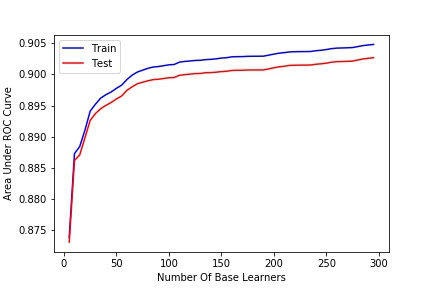
\includegraphics[scale=0.6]{adaboost.jpg}
\end{figure}
下图是RandomForest的AUC-基学习器个数折线图,可以看到训练集很快就近乎完美,测试集性能上升不如AdaBoost平稳,并且大约130个分类器就达到收敛。
\begin{figure}[H]
	\centering
	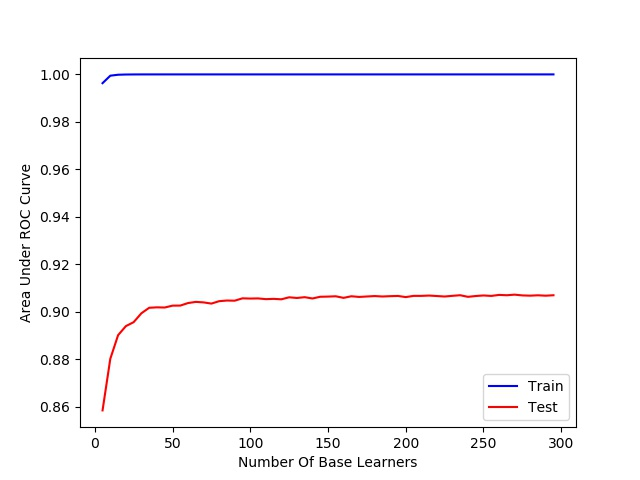
\includegraphics[scale=0.6]{randomforest.jpg}
\end{figure}
对于AdaBoost取定基学习器个数为120,得到分类器在训练集上训练之后,测试集AUC为0.8940。对于RandomForest取定基学习器个数为130,得到结果为0.9047。综合来看,RandomForest略优于AdaBoost。
\end{document}